%%%%%%%%%%%%%%%%%%%%%%%%%%%%%%%%%%%%%%%%%
% Beamer Presentation
% LaTeX Template
% Version 1.0 (10/11/12)
%
% This template has been downloaded from:
% http://www.LaTeXTemplates.com
%
% License:
% CC BY-NC-SA 3.0 (http://creativecommons.org/licenses/by-nc-sa/3.0/)
%
%%%%%%%%%%%%%%%%%%%%%%%%%%%%%%%%%%%%%%%%%

%----------------------------------------------------------------------------------------
%	PACKAGES AND THEMES
%----------------------------------------------------------------------------------------

\documentclass{beamer}

\mode<presentation> {

% The Beamer class comes with a number of default slide themes
% which change the colors and layouts of slides. Below this is a list
% of all the themes, uncomment each in turn to see what they look like.

%\usetheme{default}
%\usetheme{AnnArbor}
%\usetheme{Antibes}
%\usetheme{Bergen}
%\usetheme{Berkeley}
%\usetheme{Berlin}
%\usetheme{Boadilla}
%\usetheme{CambridgeUS}
%\usetheme{Copenhagen}
%\usetheme{Darmstadt}
%\usetheme{Dresden}
%\usetheme{Frankfurt}
%\usetheme{Goettingen}
%\usetheme{Hannover}
%\usetheme{Ilmenau}
%\usetheme{JuanLesPins}
%\usetheme{Luebeck}
\usetheme{Madrid}
%\usetheme{Malmoe}
%\usetheme{Marburg}
%\usetheme{Montpellier}
%\usetheme{PaloAlto}
%\usetheme{Pittsburgh}
%\usetheme{Rochester}
%\usetheme{Singapore}
%\usetheme{Szeged}
%\usetheme{Warsaw}

% As well as themes, the Beamer class has a number of color themes
% for any slide theme. Uncomment each of these in turn to see how it
% changes the colors of your current slide theme.

%\usecolortheme{albatross}
%\usecolortheme{beaver}
%\usecolortheme{beetle}
%\usecolortheme{crane}
%\usecolortheme{dolphin}
%\usecolortheme{dove}
%\usecolortheme{fly}
%\usecolortheme{lily}
%\usecolortheme{orchid}
%\usecolortheme{rose}
%\usecolortheme{seagull}
%\usecolortheme{seahorse}
%\usecolortheme{whale}
%\usecolortheme{wolverine}

%\setbeamertemplate{footline} % To remove the footer line in all slides uncomment this line
%\setbeamertemplate{footline}[page number] % To replace the footer line in all slides with a simple slide count uncomment this line

%\setbeamertemplate{navigation symbols}{} % To remove the navigation symbols from the bottom of all slides uncomment this line
}

\usepackage{graphicx} % Allows including images
\usepackage{booktabs} % Allows the use of \toprule, \midrule and \bottomrule in tables
\usepackage[slovene]{babel}
\usepackage[utf8]{inputenc}
\usepackage{bbm}

%----------------------------------------------------------------------------------------
%	TITLE PAGE
%----------------------------------------------------------------------------------------

\title[Classifying cyphertexts]{Classifying cyphertexts} % The short title appears at the bottom of every slide, the full title is only on the title page

\author{Rok Ivanšek} % Your name
\institute[FMF, FRI] % Your institution as it will appear on the bottom of every slide, may be shorthand to save space
{
Univerza v Ljubljani \\ % Your institution for the title page
\medskip
%\textit{john@smith.com} % Your email address
}
\date{\today} % Date, can be changed to a custom date

\begin{document}

\begin{frame}
\titlepage % Print the title page as the first slide
\end{frame}

\begin{frame}
\frametitle{Pregled} % Table of contents slide, comment this block out to remove it
\begin{itemize}
	\item Motivation
	\item Plan
	\begin{itemize}
		\item Choosing texts
		\item Procesing of texts
		\item Encrypting texts
		\item Feature engineering
		\item ML techniques
		\item Extra
	\end{itemize}
%	\item Kako se primerja z ostalimi metodami za gručenje
%	\item Praktična uporaba: nenadzorovana klasifikacija besedil
\end{itemize}
\end{frame}
%
%%----------------------------------------------------------------------------------------
%%	PRESENTATION SLIDES
%%----------------------------------------------------------------------------------------
%
%%------------------------------------------------
%\section{First Section} % Sections can be created in order to organize your presentation into discrete blocks, all sections and subsections are automatically printed in the table of contents as an overview of the talk
%%------------------------------------------------
%
%\subsection{Subsection Example} % A subsection can be created just before a set of slides with a common theme to further break down your presentation into chunks
%
%\begin{frame}
%\frametitle{Paragraphs of Text}
%Sed iaculis dapibus gravida. Morbi sed tortor erat, nec interdum arcu. Sed id lorem lectus. Quisque viverra augue id sem ornare non aliquam nibh tristique. Aenean in ligula nisl. Nulla sed tellus ipsum. Donec vestibulum ligula non lorem vulputate fermentum accumsan neque mollis.\\~\\
%
%Sed diam enim, sagittis nec condimentum sit amet, ullamcorper sit amet libero. Aliquam vel dui orci, a porta odio. Nullam id suscipit ipsum. Aenean lobortis commodo sem, ut commodo leo gravida vitae. Pellentesque vehicula ante iaculis arcu pretium rutrum eget sit amet purus. Integer ornare nulla quis neque ultrices lobortis. Vestibulum ultrices tincidunt libero, quis commodo erat ullamcorper id.
%\end{frame}

%------------------------------------------------

\begin{frame}
\frametitle{Motivation}

\begin{columns}[onlytextwidth]
  \begin{column}{0.3\textwidth}
  	\begin{figure}
		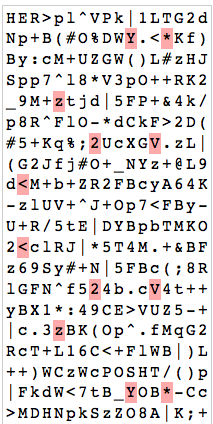
\includegraphics[scale=0.3]{cyphertext.png}
		%\caption{savate combat}
		\centering
	\end{figure}
  \end{column}
  
  \begin{column}{0.7\textwidth}
  	\pause
  	\begin{block}{}
  		Cyphertexts are unreadable.
  	\end{block}
  	
  	\pause
  	\begin{block}{}
  		Patterns can be found in cyphertexts.
  	\end{block}
  	
  	\pause
  	\begin{block}{}
  		Are the patterns clear enought to allow for a good classification model?
  	\end{block}
  \end{column}
\end{columns}

\end{frame}

%------------------------------------------------

\begin{frame}
\frametitle{Choosing texts, preprocessing, encrypting}

\begin{figure}
	
\includegraphics[scale=0.2]{data.jpg}
	%\caption{savate combat}
	\centering
\end{figure}

\begin{block}{}
\begin{itemize}
	\pause
	\item 20newsgroups corpus
	\pause
	\item Length of texts
	\pause
	\item Preprocessing steps
	\pause
	\item Choosing encryption algorithms
	\pause
	\item Raw data for modeling
\end{itemize}
\end{block}


\end{frame}



\begin{frame}
\frametitle{Feature engineering}
\begin{itemize}
	\pause
	\item This is the most difficult task of this project
	\pause
	\item Features can make or break a model
	\pause
	\item Examples of features
\end{itemize}

\pause
\begin{figure}
	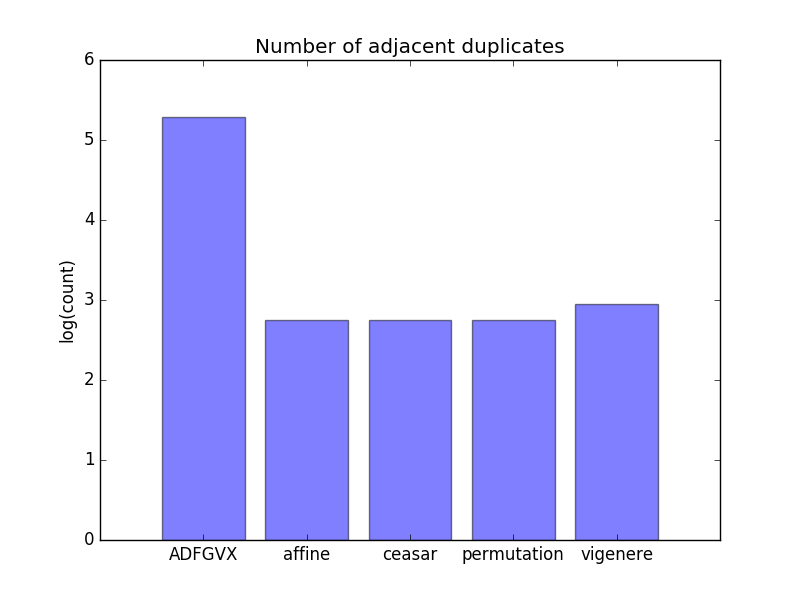
\includegraphics[scale=0.4]{no_adj_dups.png}
	%\caption{savate combat}
	\centering
\end{figure}


\end{frame}

\begin{frame}
\frametitle{Feature engineering}

\begin{figure}
	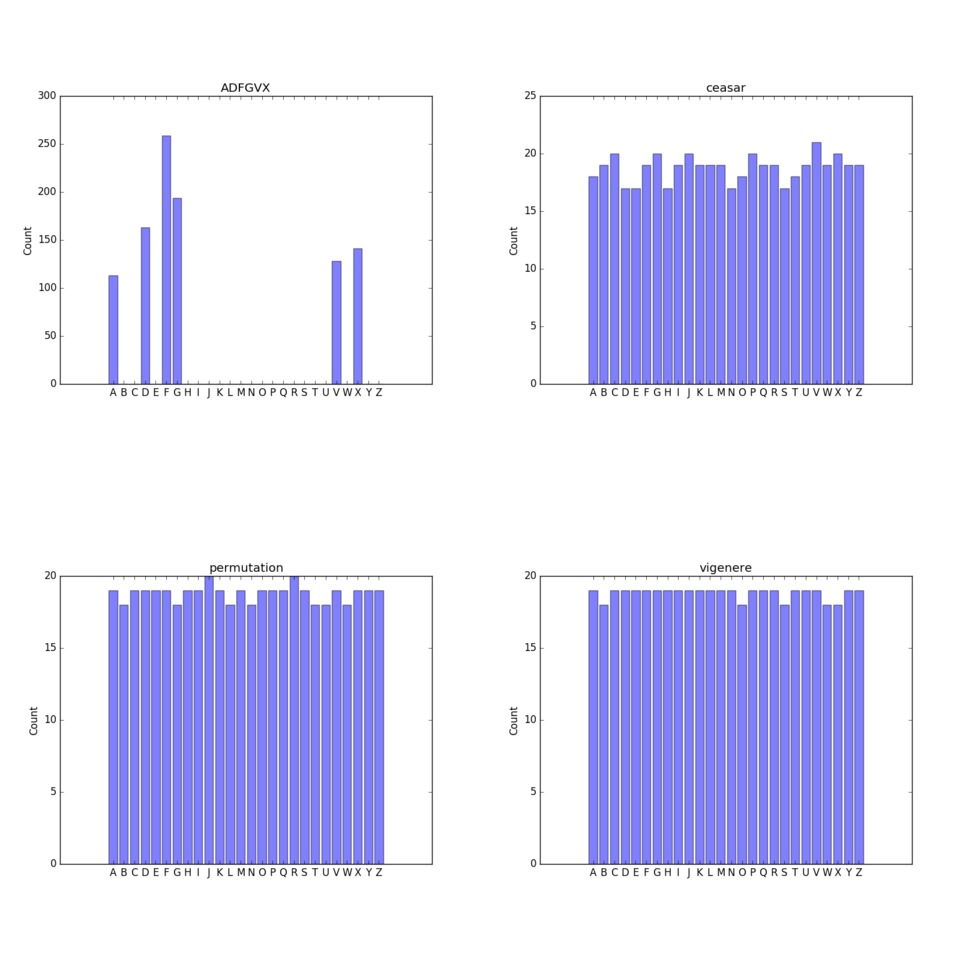
\includegraphics[width=0.6\linewidth]{montage_1.jpg}
	%\caption{savate combat}
	\centering
\end{figure}


\end{frame}

\begin{frame}
\frametitle{ML techniques, conclusion}

\pause
\begin{itemize}
	\item Random forest, Neural network
\end{itemize}

\begin{minipage}{.5\textwidth}
  \centering
  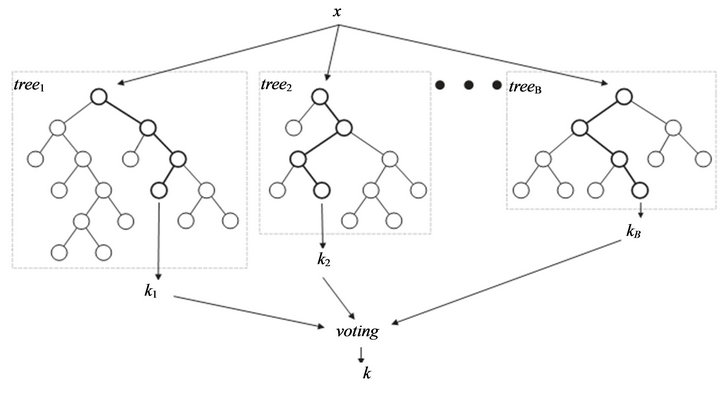
\includegraphics[width=0.8\linewidth]{random_forest.jpg}
%  \captionof{figure}{Linear model for the first dataset}
  \label{fig:test1}
\end{minipage}%
\begin{minipage}{.5\textwidth}
  \centering
  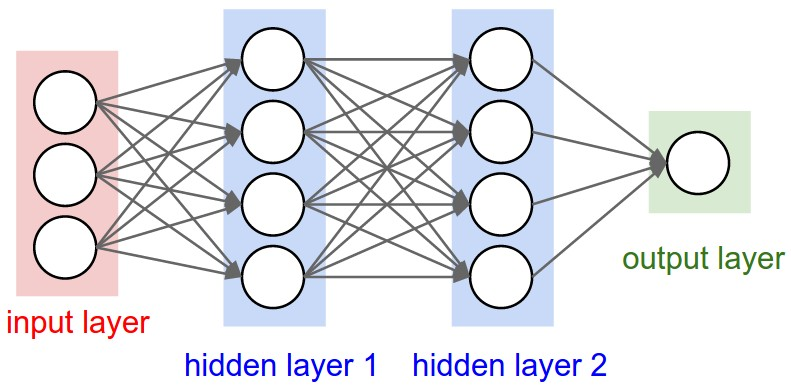
\includegraphics[width=1\linewidth]{neural_net2.jpeg}
%  \captionof{figure}{Approximating a non-linear function}
  \label{fig:test2}
\end{minipage}

\begin{itemize}
	\pause
	\item Test the model
	\pause
	\item Meassure accuracy
	\pause
	\item Try on more complicated, modern cyphers
\end{itemize}

\end{frame}
%
%\begin{frame}
%\frametitle{Lastnosti $L$}
%
%Matrika $L$ ima naslednje lastnosti:
%\begin{enumerate}
%	\pause
%	\item Za poljuben vektor $f \in \mathbb{R}^{n}$ velja
%	$$f^{'}Lf = \frac{1}{2}\sum_{i,j=1}^{n}w_{ij}(f_{i} - f_{j})^{2}.$$
%	\pause
%	\item $L$ je simetrična in pozitivno semi-definitna.
%	\pause
%	\item Najmanjša lastna vrednost $L$ je $0$ in pripadajoči lastni vektor je vektor enic $\mathbbm{1}$
%	\pause
%	\item $L$ ima $n$ nenegativnih, realnih lastnih vrednosti $0 = \lambda_{1} \leq \lambda_{2} \leq ... \leq \lambda_{n}$
%\end{enumerate}
%
%\pause
%\begin{block}{Število povezanih komponent in spekter $L$}
%Naj bo $G$ neusmerjen graf z nenegativnimi utežmi. Potem je večkratnost $k$ lastne vrednosti $0$ matrike $L$ enaka številu povezanih komponent $A_{1}, ... ,A_{k}$ grafa. Lastni prostor lastne vrednosti $0$ napenjajo vektorji enic $\mathbbm{1}_{A_{1}}, ... , \mathbbm{1}_{A_{k}}$.
%\end{block}
%\end{frame}
%
%\begin{frame}
%
%\frametitle{Lastnosti $L_{sym}$ in $L_{rw}$}
%
%\begin{enumerate}
%	\pause
%	\item Za poljuben vektor $f \in \mathbb{R}^{n}$ velja $f^{'}L_{sym}f = \frac{1}{2}\sum_{i,j=1}^{n}w_{ij}\Big(\frac{f_{i}}{\sqrt{d_{i}}} - \frac{f_{j}}{\sqrt{d_{j}}}\Big)^{2}.$
%	\pause
%	\item $\lambda$ je lastna vrednost $L_{rw}$ z lastnim vektorjem $u$, natanko tedaj, ko je $\lambda$ lastna vrednost $L_{sym}$ z lastnim vektrojem $w = D^{1/2}u$.
%	\pause
%	\item $\lambda$ je lastna vrednost $L_{rw}$ z lastnim vektorjem $u$, natanko tedaj, ko sta $\lambda$ in $u$ rešitvi enačbe $Lu = \lambda Du$.
%	\pause
%	\item $0$ je lastna vrednost $L_{rw}$ z lastnim vektorjem $\mathbbm{1}$. $0$ je lastna vrednost $L_{sym}$ z lastnim vektrojem $D^{1/2} \mathbbm{1}$.
%	\pause
%	\item $L_{sym}$ in $L_{rw}$ sta pozitivno semi-definitni in imata $n$ nenegativnih, realnih lastnih vrednosti $0 = \lambda_{1} \leq \lambda_{2} \leq ... \leq \lambda_{n}$.
%\end{enumerate}
%
%\pause
%\begin{block}{Število povezanih komponent in spekter $L_{sym}$ in $L_{rw}$}
%Naj bo $G$ neusmerjen graf z nenegativnimi utežmi. Potem je večkratnost $k$ lastne vrednosti $0$ matrik $L_{sym}$ in $L_{rw}$ enaka številu povezanih komponent $A_{1}, ... ,A_{k}$ grafa. Za $L_{rw}$, lastni prostor lastne vrednosti $0$ napenjajo vektorji enic $\mathbbm{1}_{A_{i}}$ teh komponent. Za $L_{sym}$ pa vektorji $D^{1/2}\mathbbm{1}_{A_{i}}$.
%\end{block}
%\end{frame}
%
%\begin{frame}
%\frametitle{Algoritmi spektralnega gručenja}
%
%Nenormalizirano spektralno gručenje
%
%\begin{itemize}
%\item[\bf In:] Množica ``točk''  $x_{1}, ... ,x_{n} \in \mathbb{R}^{m}$, $k$ - število gruč, ki jih želimo najti. 
%\item Skonstruiramo enega izmed grafov podobnosti. Naj bo $W$ matrika uteži. 
%\item Izračunamo nenormalizirano Laplaceovo matriko $L$.
%\item Izračunamo prvih $k$ lastnih vektrojev $u_{1},\hdots,u_{k}$ matrike $L$.
%\item Naj bo $U \in \mathbb{R}^{n \times k}$ matrika, ki ima vektroje $u_{1},\hdots,u_k$ za stolpce.
%\item Za $i=1,\hdots,n$, naj bo $y_i \in \mathbb{R}^{k}$ vektor, ki pripada $i$-ti vrstici matrike $U$.
%\item Zgručimo točke $(y_i)_{i=1,\hdots,n} \in \mathbb{R}^k$ z $k$-means algoritmom v gruče $C_1,\hdots,C_k$.
%\item[\bf Out:] Gruče $A_1,\hdots,A_k$, kjer $A_i = \{j | \; y_j \in C_i\}$.
%\end{itemize}
%	
%
%\end{frame}
%
%\begin{frame}
%\frametitle{Algoritmi spektralnega gručenja}
%
%Normalizirano spektralno gručenje (Shi, Malik (2000))
%
%\begin{itemize}
%\item[\bf In:] Množica ``točk''  $x_{1}, ... ,x_{n} \in \mathbb{R}^{m}$, $k$ - število gruč, ki jih želimo najti. 
%\item Skonstruiramo enega izmed grafov podobnosti. Naj bo $W$ matrika uteži. 
%\item Izračunamo nenormalizirano Laplaceovo matriko $L_{rw}$.
%\item Izračunamo prvih $k$ generaliziranih lastnih vektrojev $u_{1},\hdots,u_{k}$ (Pripadajoči lastnim vrednostim , ki rešijo enačbo $Lu = \lambda Du$).
%\item Naj bo $U \in \mathbb{R}^{n \times k}$ matrika, ki ima vektroje $u_{1},\hdots,u_k$ za stolpce.
%\item Za $i=1,\hdots,n$, naj bo $y_i \in \mathbb{R}^{k}$ vektor, ki pripada $i$-ti vrstici matrike $U$.
%\item Zgručimo točke $(y_i)_{i=1,\hdots,n} \in \mathbb{R}^k$ z $k$-means algoritmom v gruče $C_1,\hdots,C_k$.
%\item[\bf Out:] Gruče $A_1,\hdots,A_k$, kjer $A_i = \{j | \; y_j \in C_i\}$.
%\end{itemize}
%	
%
%\end{frame}
%
%\begin{frame}
%\frametitle{Algoritmi spektralnega gručenja}
%
%Normalizirano spektralno gručenje (Ng, Jordan, Weiss (2002))
%
%\begin{itemize}
%\item[\bf In:] Množica ``točk''  $x_{1}, ... ,x_{n} \in \mathbb{R}^{m}$, $k$ - število gruč, ki jih želimo najti. 
%\item Skonstruiramo enega izmed grafov podobnosti. Naj bo $W$ matrika uteži. 
%\item Izračunamo normalizirano Laplaceovo matriko $L_{sym}$.
%\item Izračunamo prvih $k$ lastnih vektrojev $u_{1},\hdots,u_{k}$ matrike $L_{sym}$.
%\item Naj bo $U \in \mathbb{R}^{n \times k}$ matrika, ki ima vektroje $u_{1},\hdots,u_k$ za stolpce.
%\item Iz $U$ skonstruiramo matriko $T \in \mathbb{R}^{n \times k}$, tako, da normaliziramo vrstice matrike $U$ ( $t_{ij} = u_{ij}/ \sum_{k} u_{ik}^{1/2}$).
%\item Za $i=1,\hdots,n$, naj bo $y_i \in \mathbb{R}^{k}$ vektor, ki pripada $i$-ti vrstici matrike $T$.
%\item Zgručimo točke $(y_i)_{i=1,\hdots,n} \in \mathbb{R}^k$ z $k$-means algoritmom v gruče $C_1,\hdots,C_k$.
%\item[\bf Out:] Gruče $A_1,\hdots,A_k$, kjer $A_i = \{j | \; y_j \in C_i\}$.
%\end{itemize}
%
%\end{frame}
%	
%\begin{frame}
%\frametitle{Zgled - IRIS: Opis podatkovne množice}
%
%
%\begin{itemize}
%	\item Ronald Fisher 1936
%	\item 3 vrste rož (cvetov), 50 vzorcev vsake, (setosa, versicolor, virginica)
%	\item 4 atributi, versicolor in virginica sta precej korelirani
%\end{itemize}
%
%\begin{minipage}{.3\textwidth}
%  \centering
%  \includegraphics[width=0.8\linewidth]{Iris_setosa}
%%  \captionof{figure}{Linear model for the first dataset}
%  \label{fig:test1}
%\end{minipage}%
%\begin{minipage}{.3\textwidth}
%  \centering
%  \includegraphics[width=1\linewidth]{Iris_versicolor}
%%  \captionof{figure}{Approximating a non-linear function}
%  \label{fig:test2}
%\end{minipage}
%\begin{minipage}{.3\textwidth}
%  \centering
%  \includegraphics[width=1\linewidth]{Iris_virginica}
%%  \captionof{figure}{Approximating a non-linear function}
%  \label{fig:test3}
%\end{minipage}
%
%\end{frame}	
%	
%
%\begin{frame}
%\frametitle{Zgled - IRIS}
%\begin{figure}[H]
%\centering
%\begin{minipage}{.5\textwidth}
%  \centering
%  \includegraphics[width=1.2\linewidth]{iris3d}
%%  \captionof{figure}{Linear model for the first dataset}
%  \label{fig:test1}
%\end{minipage}%
%\begin{minipage}{.5\textwidth}
%  \centering
%  \includegraphics[width=1\linewidth]{iris2d}
%%  \captionof{figure}{Approximating a non-linear function}
%  \label{fig:test2}
%\end{minipage}
%\end{figure}
%\end{frame}
%
%\begin{frame}
%\frametitle{Zgled - IRIS: Graf podobnosti}
%\begin{figure}
%	\includegraphics[scale=0.45]{iris_sim_graph}
%	%\caption{savate combat}
%	\centering
%\end{figure}
%\end{frame}
%
%\begin{frame}
%\frametitle{Zgled - IRIS: Predikcija in pravi razredi}
%
%\begin{figure}[H]
%\centering
%\begin{minipage}{.5\textwidth}
%  \centering
%  \includegraphics[width=1\linewidth]{iris_corr_clust}
%%  \captionof{figure}{Linear model for the first dataset}
%  \label{fig:test1}
%\end{minipage}%
%\begin{minipage}{.5\textwidth}
%  \centering
%  \includegraphics[width=1\linewidth]{iris_iden_clust}
%%  \captionof{figure}{Approximating a non-linear function}
%  \label{fig:test2}
%\end{minipage}
%\end{figure}
%
%\end{frame}
%
%\begin{frame}
%\frametitle{Zgled - IRIS: Točke v novem prostoru}
%\begin{figure}
%	\includegraphics[scale=0.45]{iris_new_rep}
%	%\caption{savate combat}
%	\centering
%\end{figure}
%\end{frame}
%
%\begin{frame}
%\frametitle{Zgled - IRIS: Lastne vrednosti in lastni vektorji}
%
%Lastne vrednosti:
%\begin{itemize}
%	\item 1. lastna vrednost: $-2.23567562e-15$
%	\item 2. lastna vrednost: $3.15903004e-15$
%	\item 3. lastna vrednost: $8.43897995e-01$
%\end{itemize}
%
%Lastni vektorji:\\
%\begin{minipage}{.33\textwidth}
%  \centering
%  \includegraphics[width=1\linewidth]{lv1}
%%  \captionof{figure}{Linear model for the first dataset}
%  \label{fig:test1}
%\end{minipage}%
%\begin{minipage}{.33\textwidth}
%  \centering
%  \includegraphics[width=1\linewidth]{lv2}
%%  \captionof{figure}{Approximating a non-linear function}
%  \label{fig:test2}
%\end{minipage}
%\begin{minipage}{.33\textwidth}
%  \centering
%  \includegraphics[width=1\linewidth]{lv3}
%%  \captionof{figure}{Approximating a non-linear function}
%  \label{fig:test3}
%\end{minipage}
%
%\end{frame}


%\begin{frame}
%\frametitle{Blocks of Highlighted Text}
%\begin{block}{Block 1}
%Lorem ipsum dolor sit amet, consectetur adipiscing elit. Integer lectus nisl, ultricies in feugiat rutrum, porttitor sit amet augue. Aliquam ut tortor mauris. Sed volutpat ante purus, quis accumsan dolor.
%\end{block}
%
%\begin{block}{Block 2}
%Pellentesque sed tellus purus. Class aptent taciti sociosqu ad litora torquent per conubia nostra, per inceptos himenaeos. Vestibulum quis magna at risus dictum tempor eu vitae velit.
%\end{block}
%
%\begin{block}{Block 3}
%Suspendisse tincidunt sagittis gravida. Curabitur condimentum, enim sed venenatis rutrum, ipsum neque consectetur orci, sed blandit justo nisi ac lacus.
%\end{block}
%\end{frame}
%
%%------------------------------------------------
%
%\begin{frame}
%\frametitle{Multiple Columns}
%\begin{columns}[c] % The "c" option specifies centered vertical alignment while the "t" option is used for top vertical alignment
%
%\column{.45\textwidth} % Left column and width
%\textbf{Heading}
%\begin{enumerate}
%\item Statement
%\item Explanation
%\item Example
%\end{enumerate}
%
%\column{.5\textwidth} % Right column and width
%Lorem ipsum dolor sit amet, consectetur adipiscing elit. Integer lectus nisl, ultricies in feugiat rutrum, porttitor sit amet augue. Aliquam ut tortor mauris. Sed volutpat ante purus, quis accumsan dolor.
%
%\end{columns}
%\end{frame}
%
%%------------------------------------------------
%\section{Second Section}
%%------------------------------------------------
%
%\begin{frame}
%\frametitle{Table}
%\begin{table}
%\begin{tabular}{l l l}
%\toprule
%\textbf{Treatments} & \textbf{Response 1} & \textbf{Response 2}\\
%\midrule
%Treatment 1 & 0.0003262 & 0.562 \\
%Treatment 2 & 0.0015681 & 0.910 \\
%Treatment 3 & 0.0009271 & 0.296 \\
%\bottomrule
%\end{tabular}
%\caption{Table caption}
%\end{table}
%\end{frame}
%
%%------------------------------------------------
%
%\begin{frame}
%\frametitle{Theorem}
%\begin{theorem}[Mass--energy equivalence]
%$E = mc^2$
%\end{theorem}
%\end{frame}
%
%%------------------------------------------------
%
%\begin{frame}[fragile] % Need to use the fragile option when verbatim is used in the slide
%\frametitle{Verbatim}
%\begin{example}[Theorem Slide Code]
%\begin{verbatim}
%\begin{frame}
%\frametitle{Theorem}
%\begin{theorem}[Mass--energy equivalence]
%$E = mc^2$
%\end{theorem}
%\end{frame}\end{verbatim}
%\end{example}
%\end{frame}
%
%%------------------------------------------------
%
%\begin{frame}
%\frametitle{Figure}
%Uncomment the code on this slide to include your own image from the same directory as the template .TeX file.
%%\begin{figure}
%%\includegraphics[width=0.8\linewidth]{test}
%%\end{figure}
%\end{frame}
%
%%------------------------------------------------
%
%\begin{frame}[fragile] % Need to use the fragile option when verbatim is used in the slide
%\frametitle{Citation}
%An example of the \verb|\cite| command to cite within the presentation:\\~
%
%This statement requires citation \cite{p1}.
%\end{frame}
%
%%------------------------------------------------
%



%------------------------------------------------

\begin{frame}
\Huge{\centerline{Thank you for your time}}
%\begin{figure}
%	\includegraphics[scale=0.2]{naked_man.jpg}
%	%\caption{savate combat}
%	\centering
%\end{figure}
\end{frame}

%----------------------------------------------------------------------------------------

\end{document} 